\documentclass[a4paper,11pt]{article}
	% definitions
	\author{MSC Digital Co-op}
	\title{University of Waterloo HTML Email Invitations}
	% settings
	\setlength\parindent{0pt}
	\pagestyle{headings}
	\usepackage{listings}
	\setlength{\parskip}{1em}
	\usepackage{url}
	\usepackage{enumitem}
	\setlist{leftmargin=0.75in}
	\usepackage{xcolor}
	\usepackage{mathtools}
	\usepackage{tipa}
	\lstdefinestyle{base}{
		language=Java,
		emptylines=1,
		breaklines=true,
		showstringspaces=false,
		basicstyle=\ttfamily\color{black},
		moredelim=**[is][\color{red}]{@}{@},
	}
	
	\begin{document}
	
	\maketitle %title
	\tableofcontents
	\listoffigures
	\listoftables
	
	\newpage
	\section{Introduction}
	\subsection{What are Evites?}
	HTML invitations, or evites, are event emails created using HTML. These emails are often created using a table grid structure due to the fact that email clients do not have consistent rendering. HTML emails are made using table structures rather than divs since many email clients do not have the ability to render CSS.
	\subsection{Responsiveness}
	As the popularity of mobile devices and tablets has dramatically increased in the last decade, responsiveness has become a vital part to designing webpages. Responsiveness is achieved by various HTML elements such as media queries and percentages. This allows webpages to display properly across all types of electronic devices. HTML emails are also becoming more responsive. All the evite templates have full responsiveness unless the client is sending the evite through the email client Outlook (in which case it will become a static email).
	
	%\section{Tools and Software}
	%This section lists the tools and software you will be working with for creating evites.
	%\subsection{HTML and CSS}
	%As you might have guessed from the name of HTML invites, 
	
	\section{Workflow}
	You will be working with the Creative Services department when creating evites. Below is a little overview of the workflow that goes on between you, Creative Services, and the client in the evite process.
	\begin{itemize}
		\item[Step 1] The client requests an evite via online requisition through Creative Services. The designers at Creative Services will then design an evite for the client.
		\item[Step 2] Creative Services gets the design approved by the client. The approved design is then passed onto you. You will create an evite based on the design and test it.
		\item[Step 3] After testing, you will send the evite back to Creative Services. They will also do some testing, and send it back to you if there is anything that needs to be fixed. If everything looks well, they will send it back to the client for approval.
		\item[Step 4] The client will also do once-overs. Again, if there is anything that needs to be fixed it will be sent back to you for fixes.
		\item[Step 5] If all is well, the client will send out their new evite.
	\end{itemize}
	
	\section{Setting Up}
	Creative Services will send you the files needed for the evite. This usually consists of the header image for the evite and a PDF of the evite's final design. They should tell you \textbf{how the evite will be sent out} (via Outlook on PC, Groupmail, etc.). In addition, make sure you add the evite to the MSC-DIG Tasks Smartsheet. The following process is not set in stone, but is what has previously been done.
	\begin{itemize}
		\item[Step 1] Create a new folder locally in the Evites folder (located in Documents) and name it after the project number (e.g. C008576). Save all the files that Creative Services has sent you for the evite in this folder.
		\item[Step 2] To put this folder on the Creative Services server, we use FileZilla. FileZilla is a file transfer protocol (FTP) client. The login information for FileZilla is below in Table ~\ref{tab:log}: \par
			\begin{table}[htp]
			\begin{center}
			\label{tab:log}
			\caption{FileZilla Login Details}
			\begin{tabular}{| l | l | l | l |}
			\hline
			Host & Username & Password & Port \\ \hline
			sftp://radon.uwaterloo.ca & MSC-CSCO & \textit{password} & 22 \\ \hline
			\end{tabular}
			\end{center}
			\end{table}
		\item[Step 3] In the remote site field (middle right), enter: \begin{verbatim} /fsys1/www/creativeservices.uwaterloo.ca/evites \end{verbatim}
		\item[Step 4] Make sure that the bottom portion of FileZilla is on the tab "Queued files". Drag and drop the local folder into this portion. Right click anywhere in the Queue and select "Process Queue". You can check to see if the folder has successfully been uploaded in the remote site. Alternatively, you can create a new folder with the project's number in the evites directory and drop and drop all the files sent to you in it).
		\item[Step 5] Navigate into the folder. In the permissions column, make sure all the images have the permissions "-rw-r--r--". If they don't, right click on the image and select "file permissions". In the window that pops up, type in 664 for the numeric value (Indicated in Figure ~\ref{fig:One}).
		\begin{figure}[ht]
		\centering
		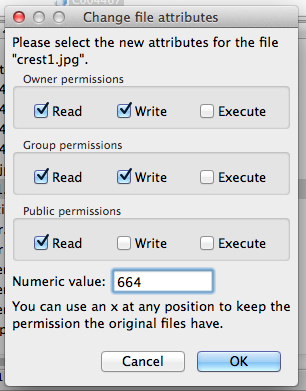
\includegraphics[width=.5\textwidth]{images/fig3}
		\caption{FileZilla Permissions}
		\label{fig:One}
		\end{figure}
	\end{itemize}
	
	\section{Outline of the Evite Process}
	\subsection{Overview of the evites}
	Although this process is not set in stone, in the past, 4 versions of the evite are created. Each version will be explained below.
	\begin{itemize}
		\item Base: this is the HTML file that you would start with from the template.
		\item Pre-inline: the version with the stylesheet contents within the head section.
		\item Online: the online version of the evite (no "Click here to view in browser", merge fields, etc). 
		\item Inline: the version with the styles all inlined in the HTML.
	\end{itemize}
	
	\section{Base: Working with the Templates}
	The templates we use are based off Zurb's Ink templates. Ink is a project launched by Zurb to provide quick and easy responsive emails. If you want to read through the documentation for the different classes, grid system, etc., visit http://zurb.com/ink/docs.php. \par
	There are 2 base templates to work from: the 1 column template and the 2 column template. Select the template that best follows the evite design that Creative Services provided to you. \par
	Open the code in any text editor or integrated development environment (IDE) you're comfortable with (if you've never used one before, Sublime Text is recommended). Then copy the contents of the template into a new file and name it after the project number.\par 
	
	Each major section of the template will be wrapped in comments that have a number and a description of what the section is for. For example,
	\begin{verbatim}
	<!-- ********************* -->
	<!-- 5 START highlight bar -->
	<!-- ********************* -->
	
	(code goes here)
	
	<!-- ***************** -->
	<!-- END highlight bar -->
	<!-- ***************** -->	
	\end{verbatim}
	All of the components are further explained below.\par
	** Note: Not all sections are in order in the code.\newpage
	
	\subsection{1 Column Template}
	\begin{center}
	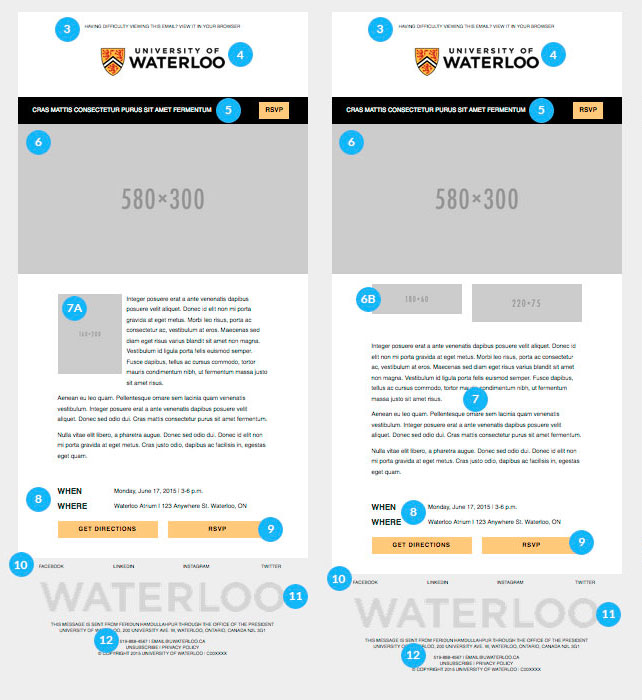
\includegraphics[scale=0.55]{images/1cols}
	\end{center}
	
	\begin{description}
		\item[3 - View in browser] \hfill \\
		This section links to the online version of the evite. Swap out instances of [job-number] in the link with the actual job number (e.g. C008840).
		\item[4 - University of Waterloo logo] \hfill \\
		The University of Waterloo logo at the top of the evite. \textbf{Do not edit this section}.
		\item[5 - Highlight bar] \hfill \\
		Contains the title of the evite and the top button. The button is styled in a "bullet-proof style", meaning that the button size will stay fixed no matter the size of the screen. Any changes made to the buttons (link, colour, size) must be made to both the commented code (for Outlook rendering) and the non-commented code.
			\begin{figure}[ht]
			\centering
			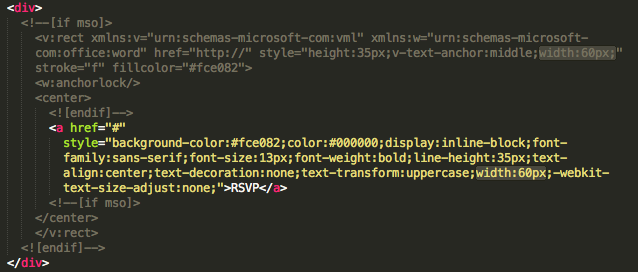
\includegraphics[width=\textwidth]{images/buttoncode}
			\caption{Bullet-proof button code}
			\label{fig:Two}
			\end{figure}
		\item[6 - Hero image] \hfill \\
		The header image for the evite. This changes for each evite. Again, the path can be obtained from FileZilla, but is usually http://creativeservices.uwaterloo.ca/evites/C00XXXX/nameoffile.jpg, where C00XXXX is the project name and nameoffile is the actual name of the header image file.
		\item[6B - Sub-images] \hfill \\
		Add the additional images in this section by un-commenting respective code in this section (left or right float or both).
		\item[7 - Body text] \hfill \\
		This is where the body text of the evite goes. When doing this section please check bolded and coloured text, as they are often links. There are also classes in the css files for faculty colours (i.e. artsorange, ahsteal, envgreen, etc) in the custom stylesheet.
		\item[7A - Optional image in text] \hfill \\
		Optional images floated to the left or right in the text content of the evite. Comment out what is not needed.
		\item[8 - Optional When/Where] \hfill \\
		You can comment this section out if it is not needed.
		\item[9 - Optional lower buttons] \hfill \\
		The links to the buttons (and sometimes the button text) is changed here. Again, you can comment these out if not needed.
		\item[10 - Social links] \hfill \\
		These usually change based on which department or faculty the evite is for.
		\item[11 - Footer logo] \hfill \\
		\textbf{Do not edit this section}.
		\item[12 - Canadian Anti-Spam Legislation (CASL) information] \hfill \\
		This information changes depending on who the client is, particularly the "Unsubscribe" link. Unless otherwise specified, the Unsubscribe button will remain as the code in 12A DEFAULT UNSUB. The other options are mostly for alumni events, news, etc. Uncomment out the version of the links that will be used and comment out the others.
	\end{description}
	
	\subsection{2 Column Template}
	\begin{center}
	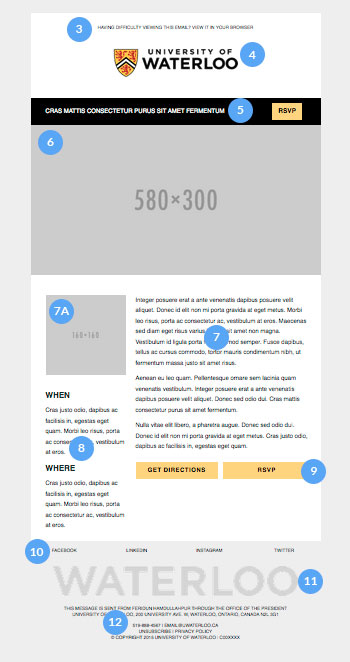
\includegraphics[scale=0.58]{images/2-col-template}
	\end{center}
	All the sections of this template are identical to the standard 1 column template, except 7A is the optional image in the left column, and 7B is the code for an optional floating image within the body text.\par
	Note that for the optional side column image, the max width of the column is \textbf{150px}.
	
	\section{Pre-inline version}
	After you are satisfied with how the evite looks, we can move on to the pre-inlined version.
	\begin{itemize}
		\item[Step 1] Select all the code (command +  A) and copy and paste it into a new file. At the top of the code in \textbf{section 1}, comment out the code that links to the stylesheets:
			\begin{verbatim}
				<link rel="stylesheet" href="../css/base.css">
				<link rel="stylesheet" href="../css/style-1-column.css">
			\end{verbatim}
		\item[Step 2] In the CSS folder, you will find the various CSS files. Copy the contents of base.css and paste it between the first style tags. \textit{It is important that the base css styles go first}.
			\begin{verbatim}
			<style type="text/css">
			/* Ink styles go here in production */
			</style>
			\end{verbatim}
		\item[Step 3] Find the css file corresponding to the template you used for the evite. Copy the contents and paste it between the second set of style tags. 
			\begin{verbatim}
			<style type="text/css">
			/* Your custom styles go here */
			</style>
			\end{verbatim}
	\end{itemize}
	This is the pre-inlined version of the evite as it no longer links to external stylesheets for the evite.
	
	\section{Online version}
	\begin{itemize}
		\item[Step 1] Copy and paste the code for the pre-inline version into a new file. Comment out \textbf{section 3} in the template (the "View in browser" link). 
		\item[Step 2] The online version of an evite should always be the links in section 12A, regardless of what the CASL links say in the non-online versions (unless otherwise specified).
		\item[Step 3] If there were any merge tags in the body content (e.g. $<$name$>$, etc.), remove it or replace it with something more general (for example, "Hello $<$name$>$," could become "Hello guest," instead). 
		\item[Step 4] Save as "C00XXXX-online.html" where C00XXXX is the project number.
		\item[Step 5] Drag and drop this file into the FileZilla folder you created for this project.
	\end{itemize}
	
	\section{Inline version}
	We need an inlined version of the HTML file because some email clients strip out $<$head$>$ and $<$style$>$ tags. 
	\begin{itemize}
		\item[Step 1] Copy the code for the pre-inline version and paste it into Ink's Inliner at http://zurb.com/ink/inliner.php. Click on ``Convert email".
		\item[Step 2] Copy the rendered code into a new file. Save as C00XXXX-inline.html.
	\end{itemize}
	This is the version of the evite we will be using to send to the client.
		
	\section{Testing}
	Testing is an important part of the evites. The testing process will depend on how the evite will be distributed (via Outlook on Mac or PC, or another email distribution service like Mailchimp or Groupmail). You will mainly be testing the inlined version, since that is the version that will be used to send out evites. 
	\subsection{Responsive and cross-browser testing}
	We want to test on various browsers/devices to ensure that the evites display properly.
	\begin{itemize}
		\item[Step 1] Open the inlined version of the evite in Chrome or Safari (Ink templates don't display properly in Firefox sometimes).
		\item[Step 2] Change the width of the browser window to ensure the responsive parts are displayed how they are supposed to.
	\end{itemize}
	
	\subsection{Testing for Outlook on PC}
	If the client is using Outlook on a PC to send out emails, you should use the PC computer behind Joe's desk to test the evite out. You will not have to test responsiveness for these emails because Outlook makes them static. Below are the steps to insert the HTML into the email.
	\begin{itemize}
		\item[Step 1] Open a new email in Outlook. Under the Insert Tab in the ribbon navigation (the top navigation), click Attachment.
		\item[Step 2] Select the inlined version of your email. Next to the Insert button, there is a little arrow. Click on that and select "Insert as text".
		\item[Step 3] Send yourself the email to see how it looks as a sent email. You might have to make a few adjustments. Repeat if necessary. You can also send the email to Jennifer or Julie at Creative Services to see if it shows up alright on their PC. 
	\end{itemize}
	** Note that forwarding evites for any reason will make extra spaces appear between sections of the evite sometimes. For best testing practice, send directly or use the Outlook template version of the evite.
	
	\subsection{Checklist for others}
	\begin{description}
		\item[Title] Make sure the Title of the document in the \texttt{$<$title$>$} tags in the \texttt{$<$head$>$} section of the HTML is changed according to the evite. 
		\item[Links] Make sure all the links are working and linking to the correct things.
		\item[Online version] Make sure the online version is linked correctly and that the link to the online version doesn't appear on the online version.
		\item[Social links] Make sure these link to the correct social media accounts.
		\item[Apostrophes and emdashes] This is mostly important for evites being sent through Groupmail. In the past, curved apostrophes and emdashes have not shown up in emails sent out through Groupmail, so we switch the curved apostrophes with a straight one (') and emdashes with hyphens.
	\end{description} \newpage

	\section{Sending out the evite}
	Again, the way the evite is prepared depends on how the client will be sending out the evite.
	\subsection{Outlook on PC}
	\begin{itemize}
		\item[Step 1] Once you get approval from Creative Services, open a new email in Outlook (on the PC). Again, insert the inlined HTML file as text into the email. At the top navigation, go to File $>$ Save As...
		\item[Step 2] Change the type of the file to Outlook template (*.oft) and save it.
		\item[Step 3] Send this file to whoever you were corresponding with in Creative Services. They will send this to the client.
	\end{itemize}
	\subsection{Outlook on Mac}
	You will be sending the inlined version to the person you were corresponding with in Creative Services. You can give these instructions to the client:
	\begin{itemize}
		\item[Step 1] Open the inlined file in either Safari or Google Chrome. Select everything (command + A) and copy it.
		\item[Step 2] Copy and paste it into the body of a new email. Fill in the rest of the fields with information (To, From, etc) and send the email.
	\end{itemize}
	\subsection{Groupmail or Mailchimp}
	For Groupmail or Mailchimp, you send the project managers in Creative services the inlined HTML file for the evite. Clients who use Groupmail should know how to take care of the rest.
	
	
	\end{document}	
	